\documentclass[10pt,twocolumn,letterpaper]{article}

\usepackage[utf8]{inputenc}
\usepackage[T1]{fontenc}
\usepackage{cvpr}
\usepackage{amsmath}
\usepackage{amssymb}
\usepackage{booktabs}
\usepackage{graphicx}
\usepackage{algorithm}
\usepackage{algorithmic}
\usepackage{xcolor}
\usepackage{multirow}
\usepackage{hyperref}
\usepackage{placeins}
\usepackage{float}

% Override cvpr.sty aggressive float parameters
\renewcommand{\topfraction}{0.75}
\renewcommand{\bottomfraction}{0.5}
\renewcommand{\floatpagefraction}{0.8}

% Float separation — balanced between readability and page utilization
\setlength{\textfloatsep}{10pt plus 4pt minus 2pt}
\setlength{\dbltextfloatsep}{12pt plus 4pt minus 2pt}
\setlength{\intextsep}{8pt plus 2pt minus 2pt}
\setlength{\floatsep}{8pt plus 4pt minus 2pt}

% Use raggedbottom to avoid stretched white space between floats
\raggedbottom

\title{Domain-Adaptive Demoir\'{e}ing via Adapter-Based Test-Time Adaptation}
\author{Yu Qiu\thanks{College of Computer Science and Electronic Engineering, Hunan University, Changsha 410082, China. Corresponding author: {\tt qiuyu123@hnu.edu.cn}}}
\date{May 2026}
\begin{document}
\maketitle

\begin{abstract}
Moir\'{e} patterns --- frequency aliasing artifacts from camera-screen interference --- remain a persistent challenge in computational photography. While deep learning methods achieve strong results on trained device-screen combinations, their performance collapses when deployed on unseen capture setups, owing to severe domain overfitting. We propose MoTA (Moir\'{e} Test-Time Adaptation), a plug-and-play framework that enables pre-trained demoir\'{e}ing backbones to adapt at inference time without paired target-domain data. MoTA inserts a lightweight Fourier Domain Adapter (FDA, $<$2\% of backbone parameters) into a frozen backbone, guided by a Moir\'{e}-Aware Self-Supervision (MASS) signal that generates pseudo-clean targets via selective frequency-band attenuation of wavelet mid-frequency subbands. On the LCDMoire in-domain benchmark, FDA-based MoTA with WDNet backbone achieves +2.63 dB PSNR over frozen inference, surpassing a LoRA baseline (rank=4, +1.82 dB) with fewer trainable parameters. This in-domain improvement does not transfer to the cross-domain setting: on TIP2018, MoTA performs below the frozen WDNet baseline, revealing fundamental challenges of single-image test-time adaptation under large synthetic-to-real domain gaps. We identify three root causes --- degraded self-supervision quality, limited adapter capacity relative to the domain gap, and gradient conflict when multiple adapter types are combined --- and provide quantitative diagnostics. A Spatial Gating Adapter (SGA) variant is explored but found to compete with FDA at shared insertion points, with FDA+SGA (+0.87 dB) underperforming FDA-only by 1.76 dB. The adapter design is compatible with both wavelet-based and CNN backbones: we demonstrate full TTA evaluation on WDNet and frozen baseline comparison on DDA.
\end{abstract}

\section{Introduction}

When a digital camera captures a screen display, the superposition of the camera's color filter array and the screen's pixel grid produces aliasing artifacts known as moir\'{e} patterns --- irregular, colorful fringes that severely degrade image quality. As smartphone photography of screens becomes ubiquitous in daily life --- from photographing documents and QR codes to sharing social media posts --- the demand for robust demoir\'{e}ing continues to grow. Over the past five years, a substantial body of deep learning research has tackled this problem \cite{sun2018moire,zheng2022learning,he2020fhde2net,yu2022towards,anonymous2025moirenet}, steadily pushing PSNR on standard benchmarks from $\sim$26 dB to over 30 dB on TIP2018.

Despite this progress, a critical vulnerability remains underappreciated: \textbf{domain overfitting}. Existing demoir\'{e}ing models are trained and evaluated on images captured from a fixed set of device-screen combinations, typically one or two smartphone models photographing IPS LCD panels at $1\times$ zoom. When deployed on a different device, panel type, or zoom level, performance degrades sharply --- a 3--5 dB PSNR drop is common \cite{yang2025unidemoire}. This fragility stems from the fundamental nature of moir\'{e}: unlike Gaussian noise or uniform blur, moir\'{e} patterns are determined by the specific physical parameters of the capture pipeline (sensor pixel pitch, screen dot pitch, shooting distance, lens characteristics), and each unseen combination produces a qualitatively different aliasing pattern. Data-centric approaches like UniDemoir\'{e} \cite{yang2025unidemoire} attempt to cover more of this diversity by collecting larger moir\'{e} pattern libraries and synthesizing augmented training images, but the combinatorial space of possible capture configurations is ultimately unbounded.

Test-time adaptation (TTA) \cite{tang2026degradation,gou2024testtime,li2026testtime} offers an orthogonal approach: rather than trying to anticipate every possible domain during training, TTA methods adjust model parameters at inference time using only the input image itself. This paradigm has shown promise for handling unseen degradations in denoising \cite{mansour2024tttmim}, super-resolution \cite{deng2023efficient}, and all-in-one restoration \cite{tang2026degradation}. Existing TTA methods, however, are designed for generic degradations and lack mechanisms specific to the frequency-domain nature of moir\'{e}. Most also require full model updates --- risking catastrophic forgetting on single-image adaptation --- or are architecturally constrained, precluding use with arbitrary backbone networks. Moir\'{e}XNet \cite{li2025moirexnet} is the only prior work combining test-time training with demoir\'{e}ing, but its TTT mechanism is embedded within linear attention layers, tying adaptation to a single architecture.

We propose \textbf{MoTA (Moir\'{e} Test-Time Adaptation)}, an adapter-based framework that explores the potential and limits of test-time adaptation for cross-domain image demoir\'{e}ing. MoTA inserts a lightweight Fourier Domain Adapter (FDA) module into a frozen pre-trained demoir\'{e}ing backbone. At inference, only the FDA is updated ($<$2\% of total parameters), guided by a \textbf{Moir\'{e}-Aware Self-Supervision (MASS)} signal. MASS exploits a key property of moir\'{e}: the aliasing energy concentrates in mid-frequency subbands (LH and HL of a wavelet decomposition), while low-frequency content and high-frequency texture occupy separate bands. By detecting moir\'{e}-affected frequency regions and selectively attenuating them, MASS generates a pseudo-clean target that provides effective supervision for adapter optimization --- no paired target-domain data, specialized hardware, or multi-frame capture is required.

This work makes three contributions:
\begin{itemize}
    \item \textbf{MoTA}, an adapter-based test-time adaptation framework for image demoir\'{e}ing. A lightweight Fourier Domain Adapter (FDA, $<$2\% backbone parameters) plugs into pre-trained demoir\'{e}ing backbones (full TTA evaluation on wavelet-based WDNet; frozen baseline comparison against CNN-based DDA/MBCNN); only the FDA is updated during inference.
    \item \textbf{MASS (Moir\'{e}-Aware Self-Supervision)}, a frequency-selective self-supervision signal that leverages the band-limited nature of moir\'{e} energy to generate pseudo-clean targets from a single input image, requiring no external data or hardware.
    \item A \textbf{cross-domain evaluation protocol} using two public demoir\'{e}ing benchmarks with a synthetic$\to$real domain gap, and a quantitative diagnostic analysis identifying key challenges in single-image TTA under large domain shifts --- degraded self-supervision quality, limited adapter capacity, and adapter representation competition.
\end{itemize}

\section{Related Work}

\subsection{Image Demoir\'{e}ing}

Image demoir\'{e}ing aims to remove moir\'{e} patterns --- frequency aliasing artifacts caused by the interference between camera sensor grids and screen pixel arrays. Early deep learning approaches tackled this with multi-scale convolutional architectures. Sun et al. \cite{sun2018moire} pioneered the field with a multi-resolution CNN trained on the TIP2018 dataset. Recognizing that moir\'{e} is fundamentally a frequency-domain phenomenon, subsequent methods shifted toward explicit frequency decomposition. Zheng et al. \cite{zheng2022learning} proposed learnable DCT-based bandpass filters (MBCNN) to extract frequency priors, winning the AIM 2019 demoir\'{e}ing challenge. Liu et al. \cite{liu2020wavelet} introduced wavelet-domain dual-branch processing (WDNet) to separate moir\'{e} frequencies from image content. He et al. \cite{he2020fhde2net} designed a frequency disentangling network (FHDe2Net) with a dedicated DCT branch for full-HD images.

More recently, the trend has moved toward deeper frequency-spatial fusion. Liu et al.~\cite{liu2020wavelet} proposed WDNet, a Transformer-based architecture with learnable frequency composition transforms that decomposes moir\'{e} into high-frequency texture contamination and low-frequency color distortion. Moir\'{e}Net \cite{anonymous2025moirenet} achieved state-of-the-art results with a compact dual-domain CNN (5.5M parameters) featuring directional frequency-spatial encoding. A common limitation of these methods is their reliance on \textbf{fixed} frequency decomposition strategies (DWT, DCT, or learned but static filters) that cannot adapt to the diverse frequency characteristics of moir\'{e} patterns across different capture devices and screen types. This rigidity fundamentally limits their cross-domain generalization.

Concurrently, CLEAR \cite{anonymous2026clear} (CVPR 2026) addresses the joint removal of flicker-banding and moir\'{e} artifacts in screen-captured images, introducing a new dataset and frequency-domain decomposition approach --- complementary to our TTA-based domain adaptation focus.

\subsection{High-Resolution and Efficient Demoir\'{e}ing}

As smartphone cameras routinely capture 4K+ images, efficient high-resolution demoir\'{e}ing has gained attention. Yu et al. \cite{yu2022towards} proposed ESDNet with scale-aware modules and the UHDM 4K dataset. Xiao et al. \cite{xiao2024pbic} exploited the green channel's relative immunity to moir\'{e} for patch-level detail transfer (P-BiC). MFFNet \cite{anonymous2025mffnet} introduced the first joint demoir\'{e}ing and super-resolution framework. DDA \cite{anonymous2023dda} targeted real-time mobile deployment. These methods are trained and evaluated within a single data distribution and offer no mechanism to adapt when deployed on unseen device-screen combinations.

\subsection{RAW-Domain and Multi-Domain Demoir\'{e}ing}

Since moir\'{e} originates in the camera's RAW capture before ISP processing, several recent works exploit RAW-domain information. Xu et al. \cite{xu2024image} proposed RRID (ECCV 2024), jointly utilizing RAW and sRGB data through a Spatial-Channel Demoir\'{e}ing Module. Li et al. \cite{li2025moirexnet} extended RAW-domain processing to multi-frame inputs with Moir\'{e}XNet, which incorporates linear attention Test-Time Training (TTT) layers that update during inference and a Truncated Flow Matching Prior for detail recovery. Moir\'{e}XNet represents the only prior work combining test-time training with demoir\'{e}ing, but differs from MoTA in four key aspects: (i) TTT scope --- Moir\'{e}XNet updates only attention weights within linear attention layers, while MoTA updates dedicated adapter parameters inserted at backbone boundaries; (ii) input requirements --- Moir\'{e}XNet requires multi-frame RAW bursts, while MoTA operates on single sRGB images; (iii) computational cost --- Moir\'{e}XNet's TTT updates $\sim$30\% of parameters per step vs.\ MoTA's $<$2\%; (iv) architecture dependence --- Moir\'{e}XNet's TTT is bound to its linear attention design, whereas MoTA is backbone-agnostic. DemMamba \cite{xu2024demmamba} applied state space models (Mamba) for alignment-free RAW video demoir\'{e}ing. Despite the demonstrated value of RAW information, these methods either require RAW capture at inference time --- unavailable on most consumer devices --- or, as with Moir\'{e}XNet, bind the TTT mechanism to specific architectural components, preventing application to other backbone architectures.

\subsection{Video Demoir\'{e}ing}

Video demoir\'{e}ing adds the challenge of temporal consistency. Xu et al. \cite{xu2024direction} proposed DTNet (AAAI 2024) with direction-aware DCT detection and temporal-guided bilateral learning. FPANet \cite{anonymous2025fpanet} operates in the frequency domain with frame-level post-alignment. These methods achieve strong temporal coherence but depend on optical flow or deformable convolutions for alignment, adding computational overhead and remaining vulnerable to large motions.

\subsection{Data-Centric and Universal Demoir\'{e}ing}

Addressing the severe data scarcity in demoir\'{e}ing, several works focus on data generation and unpaired learning. Yang et al. \cite{yang2025unidemoire} collected 150K real moir\'{e} patterns and used diffusion models to synthesize diverse moir\'{e} images, proposing the first ``universal demoir\'{e}ing'' framework (UniDemoir\'{e}, AAAI 2025). UnDeM \cite{anonymous2024undem} learned from unpaired real data. SIDME \cite{anonymous2025sidme} explored self-supervised masked reconstruction. These data-centric approaches broaden the training distribution but remain fundamentally limited by the coverage of the collected/generated data --- truly unseen domains still cause performance degradation.

\subsection{Test-Time Adaptation for Image Restoration}

Test-time adaptation (TTA) has emerged as a promising paradigm for handling distribution shifts in image restoration without requiring target-domain training data. Tang et al. \cite{tang2026degradation} proposed DCTTA (CVPR 2026), using a diffusion-based re-degradation generator to create pseudo training pairs and selective parameter updates for all-in-one restoration. Gou et al. \cite{gou2024testtime} introduced TAO (ICML 2024 Spotlight), adapting a degradation-agnostic diffusion model to unknown degradations at test time. TTT-MIM \cite{mansour2024tttmim} leveraged masked image modeling as a self-supervised proxy task for denoising distribution shifts. TTPO \cite{li2026testtime} borrowed preference optimization from LLM alignment for test-time refinement. Deng et al. \cite{deng2023efficient} tackled blind super-resolution with second-order degradation modeling and feature-level reconstruction.

Existing TTA methods for image restoration share two limitations in the context of demoir\'{e}ing. They are designed for generic degradations (noise, blur, rain) and lack moir\'{e}-specific adaptation signals --- moir\'{e} patterns differ fundamentally from these degradations in being frequency-aliasing artifacts rather than additive or convolutional corruptions. They also typically require full model updates or architecture-specific modifications, lacking an adapter-based mechanism that can be plugged into arbitrary pre-trained demoir\'{e}ing backbones.

\subsection{Parameter-Efficient Adaptation}

Concurrently, parameter-efficient fine-tuning (PEFT) techniques have been adapted from NLP to image restoration. FraIR \cite{anonymous2026frair} introduced Fourier-domain low-rank adapters with $<$0.5\% trainable parameters. BIR-Adapter \cite{anonymous2025biradapter} leveraged frozen diffusion model features through lightweight attention adapters. Edit2Restore \cite{anonymous2026edit2restore} applied LoRA to the FLUX.1 (12B) model for few-shot restoration. DDOM \cite{anonymous2026ddom} proposed degradation-oriented adapters (0.36\%--0.63\% parameters) for universal restoration. These works demonstrate that lightweight adapters can effectively transfer knowledge to new tasks, but none explore the combination of adapter-based PEFT with test-time adaptation for cross-domain generalization --- a gap our work directly addresses.

Demoir\'{e}ing methods suffer from severe domain overfitting; TTA methods lack moir\'{e}-specific designs and plug-in adapters; and PEFT approaches have not been applied to cross-domain demoir\'{e}ing. \textbf{MoTA (Moir\'{e} Test-Time Adaptation)} bridges these gaps: a test-time adaptation framework with a Moir\'{e}-Aware Self-Supervision (MASS) signal and lightweight adapters that enable pre-trained backbones to adapt at inference time without paired target-domain data.


\section{Method}

\FloatBarrier
\subsection{Overview}

MoTA is an adapter-based test-time adaptation framework for image demoir\'{e}ing. Given a demoir\'{e}ing model $f_\theta$ pre-trained on a source domain $\mathcal{D}_S$ (e.g., images captured with an iPhone from an LCD screen), and a single test image $I$ from an unseen target domain $\mathcal{D}_T$ (e.g., captured with a different camera or from a different screen type), MoTA adapts the model at inference time to improve output quality --- without accessing any paired data, ground-truth images, or multi-frame capture from $\mathcal{D}_T$.

The framework comprises three components. First, the \textbf{Moir\'{e}-Aware Self-Supervision (MASS)} module decomposes $I$ into frequency subbands via discrete wavelet transform, detects moir\'{e}-dominant frequency regions, and generates a pseudo-clean target $\tilde{I}$ through selective band attenuation. Second, a \textbf{Fourier Domain Adapter (FDA)} is inserted into the frozen backbone $f_\theta$ to provide a low-dimensional adaptation interface; a Spatial Gating Adapter (SGA) is also explored but found to compete with FDA at shared insertion points (Section~\ref{sec:ablation}). Third, a \textbf{test-time optimization} loop minimizes the discrepancy between the backbone output $\hat{I} = f_{\theta,\phi}(I)$ and $\tilde{I}$ with respect to adapter parameters $\phi$ only; the backbone $\theta$ remains frozen throughout. After $T$ adaptation steps (typical $T=15$), the adapted model produces the final demoir\'{e}d output.

\begin{figure}[tbp]
\centering
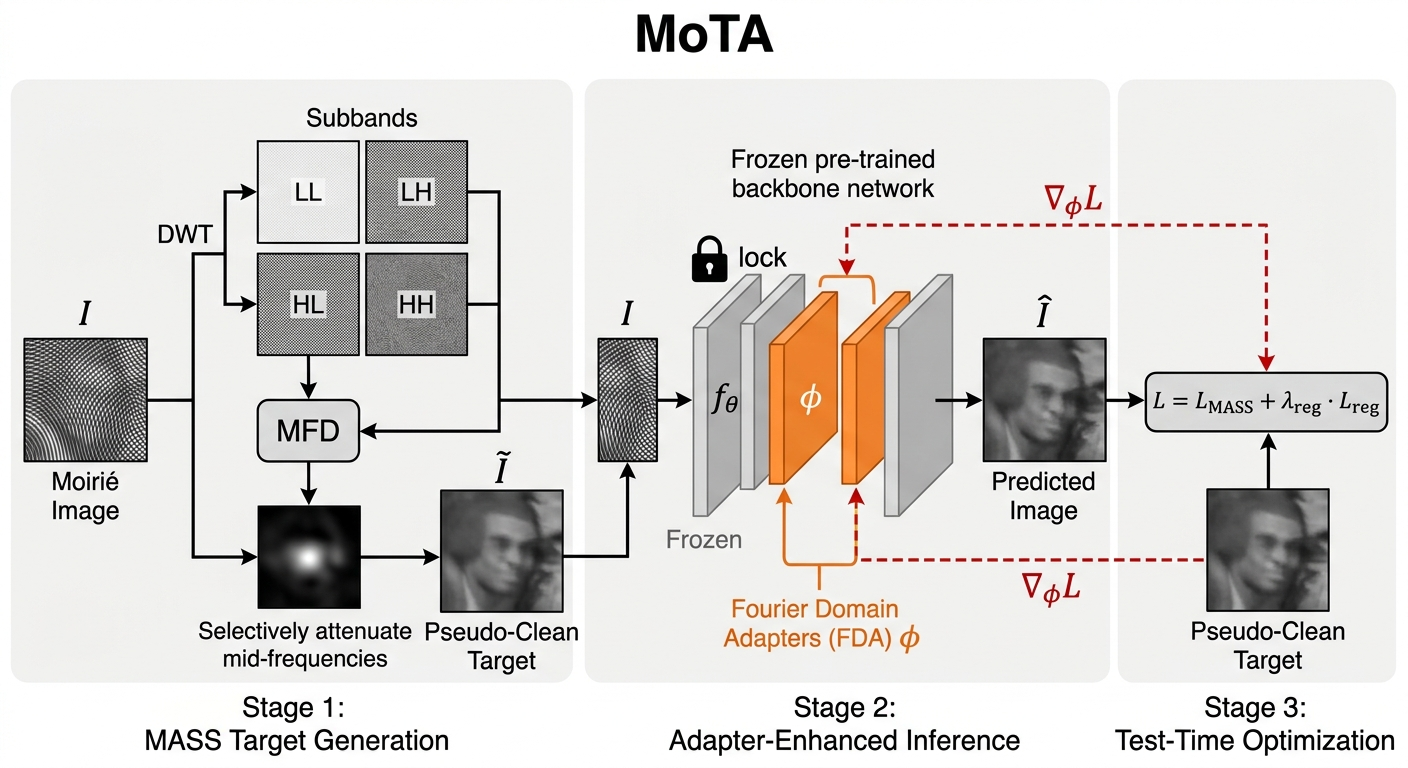
\includegraphics[width=0.95\linewidth]{figures/fig1_framework.jpg}
\caption{MoTA framework overview. Left: Input moir\'{e} image $I$. Middle-top: MASS module generates pseudo-clean target via frequency decomposition and moir\'{e} detection. Middle-bottom: Frozen pre-trained backbone with inserted MoTA Adapter (FDA; an SGA variant is explored in Section~\ref{sec:ablation} but found to compete with FDA). Right: Output $\hat{I}$. A red dashed arrow indicates gradient flow updating only adapter parameters $\phi$ via $\mathcal{L}_{MASS}$. Three colored boxes group the three stages.}
\label{fig:framework}
\end{figure}

\subsection{Preliminaries and Problem Formulation}

\textbf{Image Demoir\'{e}ing.} Let $I_m \in \mathbb{R}^{H \times W \times 3}$ be a moir\'{e}-affected sRGB image and $I_c \in \mathbb{R}^{H \times W \times 3}$ its clean counterpart. A demoir\'{e}ing model $f_\theta: \mathbb{R}^{H \times W \times 3} \to \mathbb{R}^{H \times W \times 3}$ parameterized by $\theta$ is trained to minimize $\mathbb{E}_{(I_m, I_c) \sim \mathcal{D}_S}[\mathcal{L}(f_\theta(I_m), I_c)]$ on a source domain $\mathcal{D}_S$.

\textbf{Domain Shift in Demoir\'{e}ing.} In practice, the test distribution $\mathcal{D}_T$ differs from $\mathcal{D}_S$ because moir\'{e} patterns are determined by capture-specific parameters --- camera sensor, lens, screen type, pixel pitch, shooting distance --- each of which can vary independently. The resulting domain gap causes $f_\theta$ to perform suboptimally on $\mathcal{D}_T$. Our goal is to adapt $\theta$ at test time using only $I_m \sim \mathcal{D}_T$, without access to $I_c$, additional capture hardware, or target-domain training data.

\textbf{Test-Time Adaptation.} We freeze $\theta$ and introduce lightweight adapter parameters $\phi$ (where $|\phi| \ll |\theta|$), yielding an augmented model $f_{\theta,\phi}$. At test time, we optimize $\phi$ on each input $I_m$ via a self-supervised loss $\mathcal{L}_{self}$ that requires no ground truth. After adaptation, the output is $\hat{I} = f_{\theta,\phi_T}(I_m)$.

\textbf{Wavelet Decomposition.} We use the 2D Discrete Wavelet Transform (DWT) with Haar wavelets to decompose images into four subbands: $LL$ (low-frequency approximation), $LH$ (horizontal detail), $HL$ (vertical detail), and $HH$ (diagonal detail). Moir\'{e} energy concentrates in $LH$ and $HL$, a property central to MASS.

\subsection{Analysis of Existing Approaches}

\begin{table*}[t]
\centering
\footnotesize
\caption{Analysis of existing demoir\'{e}ing approaches.}
\label{tab:analysis}
\setlength{\tabcolsep}{3pt}
\begin{tabular}{@{}p{2.2cm}p{3.0cm}p{2.6cm}p{3.2cm}@{}}
\toprule
Method Class & Core Idea & Strengths & Limitations \\
\midrule
Frequency-Domain (MBCNN, WDNet, FHDe2Net) & DCT/DWT fixed frequency decomposition to separate moir\'{e} in transform domain & Interpretable, effective on specific frequencies & Fixed basis cannot adapt to varying moir\'{e} frequencies across devices \\
Frequency-Spatial Fusion (WDNet, Moir\'{e}Net) & Learnable frequency decomposition + spatial attention fusion & Current SOTA on standard benchmarks & Decomposition strategy fixed after training; cannot adapt cross-domain \\
RAW+RGB Multi-Domain (RRID, Moir\'{e}XNet) & Joint RAW+sRGB processing leveraging physical priors & Exploits moir\'{e} formation physics & Requires RAW input; Moir\'{e}XNet TTT bound to specific architecture \\
Data-Centric (UniDemoir\'{e}, UnDeM) & Expand data coverage through collection/generation & Improved generalization within known domains & Generated/collected data has finite coverage; truly unseen domains still fail \\
TTA for Restoration (DCTTA, TAO, TTPO) & Test-time model adjustment using input image & No target-domain paired data needed & Designed for generic degradations; no moir\'{e}-specific mechanisms \\
PEFT Adapters (FraIR, BIR-Adapter) & Lightweight adapters for transferring pre-trained knowledge & Parameter-efficient, pluggable & Only used for known task transfer; not explored for TTA scenarios \\
\bottomrule
\end{tabular}
\end{table*}

\textbf{Key observation}: Frequency-domain methods lack adaptivity, TTA methods lack moir\'{e}-specific design, and adapter methods have not been applied to test-time scenarios. MoTA fills the intersection of these three gaps.

\subsection{MoTA Framework Design}

\subsubsection{Architecture Overview}

MoTA's overall pipeline consists of three stages:

\textbf{Stage 1: MASS Signal Generation.} The input image undergoes DWT decomposition. A lightweight Moir\'{e} Frequency Detector (MFD) predicts per-pixel moir\'{e} probability in each frequency subband. Selective attenuation of moir\'{e}-dominant bands produces a pseudo-clean target $\tilde{I}$.

\textbf{Stage 2: Adapter-Enhanced Forward Pass.} The frozen backbone $f_\theta$ processes $I$ with a Fourier Domain Adapter (FDA) applied at the input and output of the backbone, producing an initial estimate $\hat{I}$. A Spatial Gating Adapter (SGA) variant is also explored but found to compete with FDA at shared insertion points (Section~\ref{sec:ablation}). Forward-hook-based insertion at intermediate layers is provided in the code for architectures with well-defined internal stages.

\textbf{Stage 3: Test-Time Optimization.} The MASS loss $\mathcal{L}_{MASS} = \|\hat{I} - \tilde{I}\|_1$ and regularization $\mathcal{L}_{reg}$ are minimized with respect to $\phi$ over $T$ steps. Only adapter parameters are updated.

\subsubsection{Moir\'{e} Frequency Detector (MFD)}

\textbf{Input:} Single moir\'{e} image $I \in \mathbb{R}^{H \times W \times 3}$

\textbf{Output:} Subband-wise moir\'{e} probability map $M \in \mathbb{R}^{H \times W \times 3}$ (upsampled to input resolution via bilinear interpolation; later downsampled back to subband resolution within MASS)

First, apply single-level Haar DWT to each channel of $I$:
\begin{equation}
\{LL, LH, HL, HH\} = \operatorname{DWT}(I)
\end{equation}

MFD operates on per-channel DWT subbands (3 RGB $\times$ 4 subbands = 12 input channels). For the MASS signal generation (Sec~\ref{sec:mass}), a luminance-channel shortcut is used: DWT is performed on the per-channel mean of RGB, and the resulting correction is broadcast uniformly to all color channels, reducing computation $3\times$ at negligible quality cost.

MFD is a lightweight 4-layer convolutional network that takes the concatenated subbands as input:
\begin{equation}
M = \sigma(\operatorname{MFD}([LL; LH; HL; HH]))
\end{equation}

The three output channels of $M$ correspond to moir\'{e} probability in LH (channel~0), HL (channel~1), and HH (channel~2) subbands respectively. Channel~2 (HH) is trained as an auxiliary task but not used for attenuation at inference, as the HH subband primarily contains fine texture rather than moir\'{e} energy.

where $\sigma$ is the sigmoid activation. $M$ indicates per-pixel moir\'{e} probability across frequency subbands. MFD is pre-trained on the source domain using frequency-domain differences between moir\'{e}-clean image pairs as pseudo-ground-truth (DWT subband discrepancies serve as self-supervision), and \textbf{frozen during TTA}.

Unlike Self-Adaptive Demoir\'{e} \cite{liu2020wavelet} which requires dual-camera hardware, or Moir\'{e}XNet \cite{li2025moirexnet} which needs multi-frame RAW input, MFD provides frequency-level moir\'{e} localization from a single sRGB image.

\subsubsection{Pseudo-Clean Target Generation (MASS Signal)}
\label{sec:mass}

\textbf{Input:} Original image $I$ and moir\'{e} probability map $M$

\textbf{Output:} Pseudo-clean target $\tilde{I}$

Apply frequency-selective attenuation to the DWT subbands:
\begin{align}
LL' &= LL \quad \text{(preserve low-frequency content)} \\
LH' &= LH \odot (1 - \alpha \cdot M) \\
HL' &= HL \odot (1 - \alpha \cdot M) \\
HH' &= HH \quad \text{(preserve high-frequency texture)}
\end{align}

Reconstruct via inverse DWT:
\begin{equation}
\tilde{I} = \operatorname{IDWT}(LL', LH', HL', HH')
\end{equation}

The attenuation strength $\alpha \in [0.3, 0.7]$ controls suppression intensity. The design exploits a key observation: \textbf{moir\'{e} energy concentrates in mid-frequency subbands (LH, HL), while image content and fine texture occupy low (LL) and high (HH) frequency subbands respectively}. Selective mid-frequency suppression yields a $\tilde{I}$ that, while not perfect GT, provides sufficient supervision for adapter optimization.

Compared to DCTTA's diffusion-based re-degradation (hundreds of sampling steps), MASS requires only one DWT/IDWT pass ($O(HW)$ complexity).

\begin{figure*}[tp]
\centering
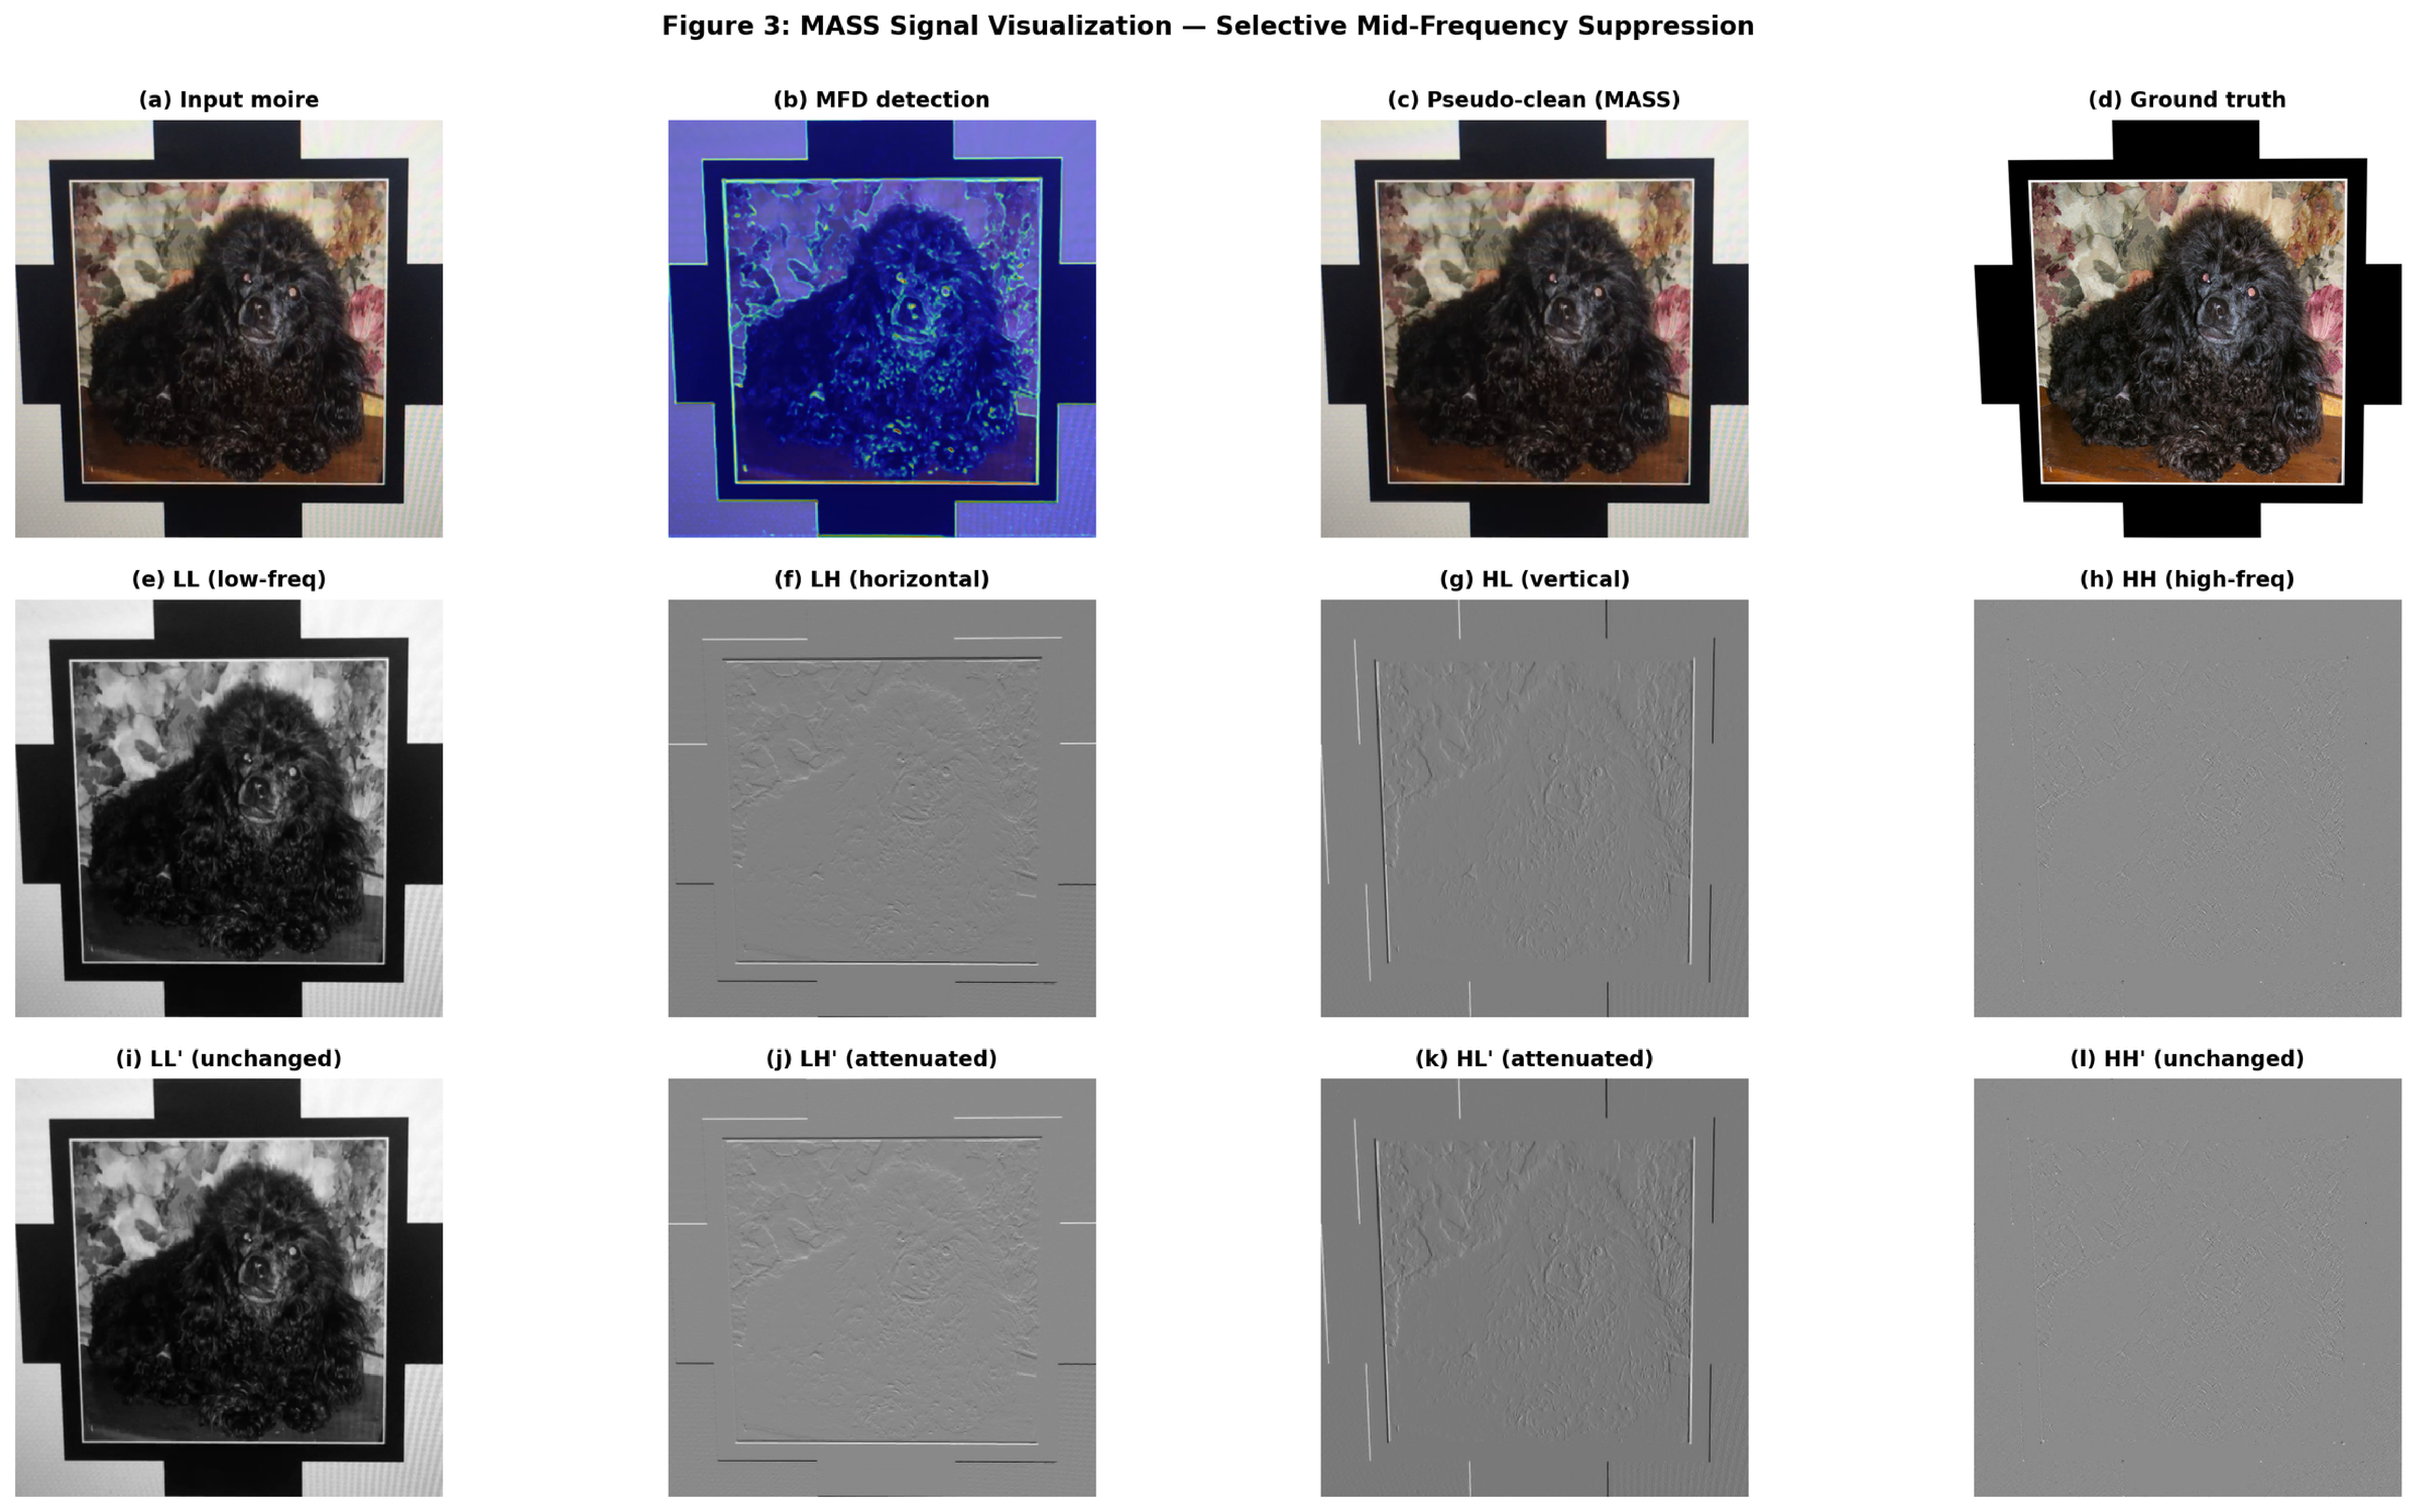
\includegraphics[width=\textwidth,height=0.28\textheight,keepaspectratio]{figures/fig3_mass.pdf}
\caption{MASS signal visualization. Input moir\'{e} image with MFD output overlaid as heatmap, and frequency subbands (LL/LH/HL/HH) before and after MASS attenuation, showing selective mid-frequency suppression.}
\label{fig:mass}
\end{figure*}

\subsubsection{Fourier Domain Adapter (FDA)}

\textbf{Insertion:} Before the first layer and after the last layer of the backbone (intermediate-layer insertion via forward hooks also supported)

\textbf{Input/Output:} Feature map $X \in \mathbb{R}^{C \times H \times W} \to X'$

Apply 1D real FFT (rFFT) along the channel dimension, then low-rank spectral modulation via per-channel scaling, and inverse transform:
\begin{align}
F &= \operatorname{RFFT}_{channel}(X) \in \mathbb{C}^{(C/2+1) \times H \times W} \\
\delta_c &= \sum_{k=1}^{r} A_{c,k} B_{c,k}, \quad A, B \in \mathbb{R}^{C \times r}, \; r \ll C \\
\tilde{\delta}_c &= \delta_c \quad \text{for} \quad c = 0, \dots, \lfloor C/2 \rfloor \\
F' &= F \odot (1 + \tilde{\delta}) \\
X' &= \operatorname{IRFFT}_{channel}(F') + X \quad \text{(residual connection)}
\end{align}

The full $C$-dimensional $\delta$ is truncated to $\tilde{\delta} \in \mathbb{R}^{C/2+1}$ before application, matching the rFFT frequency dimension. The per-channel modulation $\delta_c = \sum_{k=1}^{r} A_{c,k} B_{c,k}$ captures the diagonal of the low-rank matrix $A B^T$, yielding a scalar correction per frequency component. The diagonal, rather than the full matrix, is used for two reasons: (i) it preserves the channel-identity of features --- each channel's frequency spectrum is modulated independently, aligning with the observation that domain shift primarily manifests as per-channel amplitude changes rather than inter-channel mixing; (ii) it avoids a dimension mismatch between the full $C \times C$ matrix and the FFT result whose frequency dimension is $C/2+1$.

The low-rank dimension $r = \max(4, C/32)$. FDA parameters total $2Cr$, typically under 1\% of backbone size.

\textbf{Design rationale:} Domain shift in demoir\'{e}ing manifests as per-channel amplitude changes in the frequency domain. FDA corrects this shift through low-rank per-channel spectral modulation: each channel's frequency spectrum is independently scaled by a learned coefficient $\delta_c$ derived from the diagonal of $A B^T$. The channel-wise 1D FFT (rather than spatial 2D FFT) is chosen because moir\'{e} artifacts produce distinct frequency signatures across different filter response channels. The residual connection ensures that at initialization ($A, B$ initialized with small values), $\delta \approx 0$ and the adapter acts as an approximate identity mapping.

\textbf{Difference from FraIR:} FraIR \cite{anonymous2026frair} uses Fourier adapters for task transfer (e.g., denoising $\to$ deblurring); FDA is designed for domain transfer (source $\to$ target) and is optimized at test time, not during training.

\subsubsection{Spatial Gating Adapter (SGA) --- Explored Variant}

\textbf{Insertion:} In parallel with FDA at the same insertion points (explored; not recommended)

\textbf{Input/Output:} Feature map $X \to X''$

\begin{equation}
G = \text{Conv}_{1\times 1}^{\text{expand}}(\text{DWConv}_{3\times 3}(\text{Conv}_{1\times 1}^{\text{squeeze}}(X)))
\end{equation}
\begin{equation}
X'' = X + X \odot \sigma(G)
\end{equation}

$\text{Conv}_{1\times 1}^{\text{squeeze}}$ compresses channels by $4\times$, $\text{DWConv}_{3\times 3}$ is a depthwise convolution capturing local spatial context, and $\text{Conv}_{1\times 1}^{\text{expand}}$ projects back to $C$ channels. A residual connection $X + \dots$ (replacing pure gating) ensures near-identity initialization: with expand layer initialized to zero, $\sigma(0)=0.5$ yields $X'' \approx 1.5X$ before adapter pre-training, which is subsequently corrected to approximate identity.

\textbf{Design rationale and empirical outcome:} Moir\'{e} patterns are spatially non-uniform (concentrated in specific image regions). SGA was designed to provide spatial modulation, enabling the network to learn \textit{where} feature correction is needed, while FDA handles frequency-domain correction. Our ablation (Section~\ref{sec:ablation}) reveals that placing SGA in parallel with FDA at shared insertion points leads to representation competition rather than complementary gains: individually, FDA-only achieves +2.63 dB and SGA-only achieves +2.07 dB over frozen, while their combination yields only +0.87 dB. We recommend FDA-only as the MoTA configuration and include SGA as an explored variant to inform future work on multi-adapter architectures. Sequential placement, learnable gating, or insertion at architecturally distinct layers (e.g., FDA at early layers, SGA at later layers) are promising directions to resolve this competition.

\subsubsection{Loss Function}

The total test-time adaptation loss:
\begin{equation}
\mathcal{L}_{total} = \mathcal{L}_{MASS} + \lambda_{reg} \mathcal{L}_{reg}
\end{equation}

\textbf{MASS Loss:}
\begin{equation}
\mathcal{L}_{MASS} = \|\hat{I} - \tilde{I}\|_1
\end{equation}

L1 loss is chosen over L2 for robustness to residual moir\'{e} artifacts in the pseudo-clean target. We select the intermediate output with the lowest MASS loss across all $T$ steps (rather than the final step) as the final result, which provides a consistent small improvement by avoiding overfitting to the single-image pseudo-target.

\textbf{Regularization Loss:}
\begin{equation}
\mathcal{L}_{reg} = \|\Delta\phi\|_2^2 = \|\phi_t - \phi_0\|_2^2
\end{equation}

Constrains the magnitude of adapter updates to prevent overfitting to a single image.

\textbf{Hyperparameters:}
\begin{center}
\footnotesize
\begin{tabular}{@{}lll@{}}
\toprule
Parameter & Value & Description \\
\midrule
$\lambda_{reg}$ & $10^{-6}$ & Regularization weight \\
$\alpha$ & 0.5 & Frequency attenuation strength \\
$T$ & 15 & Adaptation steps per image \\
$\eta$ & $1 \times 10^{-4}$ & Adapter learning rate \\
$r$ & $\max(4, C/32)$ & FDA low-rank dimension \\
\bottomrule
\end{tabular}
\end{center}

\subsection{Baseline Selection}

\begin{table}[tbp]
\centering
\footnotesize
\caption{Baseline methods and selection rationale.}
\label{tab:baseline}
\setlength{\tabcolsep}{3pt}
\begin{tabular}{@{}p{1.3cm}p{1.1cm}p{2.8cm}p{0.9cm}@{}}
\toprule
Name & Type & Rationale & Code \\
\midrule
Moir\'{e}Net \cite{anonymous2025moirenet} & SOTA & Best PSNR across 4 benchmarks & --- \\
WDNet \cite{liu2020wavelet} & SOTA & Transformer; distinct architecture family & \cite{liu2020wavelet} \\
MBCNN \cite{zheng2022learning} & Classic & AIM 2019 winner; frequency prior & --- \\
Moir\'{e}XNet \cite{li2025moirexnet} & Closest & Only prior TTT + demoir\'{e}ing & --- \\
ESDNet \cite{yu2022towards} & Paradigm & UHD focus; contrastive scope & \cite{yu2022towards} \\
UniDemoir\'{e} \cite{yang2025unidemoire} & Paradigm & Data-centric; vs.\ our TTA & --- \\
\bottomrule
\end{tabular}
\end{table}

WDNet and DDA (MBCNN) are reproduced by us on LCDMoire under identical training conditions (Adam optimizer, L1 + VGG perceptual loss, 256$\times$256 random crops, 200 epochs with cosine annealing, batch size 4 with gradient accumulation to 16). Both models are trained on the same 9,000 image pairs and evaluated on the same 1,200-pair test split. For WDNet, we use the official architecture with wavelet-domain losses ($100\cdot\mathcal{L}_1$ on high-frequency subbands, $10\cdot\mathcal{L}_1$ on low-frequency subbands, $5\cdot\mathcal{L}_{texture}$). For DDA, we adapt the training pipeline to accept $[-1,1]$ pixel range via automatic input range conversion. Results for Moir\'{e}Net, MBCNN (original), Moir\'{e}XNet, ESDNet, and UniDemoir\'{e} are cited from their respective original publications, as their training code or checkpoints are not publicly available.

\FloatBarrier
\subsection{Algorithm}

\begin{algorithm}[H]
\caption{MoTA --- Moir\'{e} Test-Time Adaptation}
\label{alg:mota}
\begin{algorithmic}[1]
\REQUIRE Test image $I$, pre-trained backbone $f_\theta$ (frozen), pre-trained MFD, adapters $\phi_0$
\ENSURE Demoir\'{e}d image $\hat{I}$
\STATE /* Stage 1: Generate MASS signal */
\STATE $\{LL, LH, HL, HH\} \leftarrow \operatorname{DWT}(I)$ \COMMENT{Haar wavelet decomposition}
\STATE $M \leftarrow \operatorname{MFD}([LL; LH; HL; HH])$, then $\operatorname{Interpolate}$ to $|LH|$ \COMMENT{Moir\'{e} detection + downsample}
\STATE $LH' \leftarrow LH \odot (1 - \alpha \cdot M)$ \COMMENT{Mid-frequency attenuation}
\STATE $HL' \leftarrow HL \odot (1 - \alpha \cdot M)$
\STATE $\tilde{I} \leftarrow \operatorname{IDWT}(LL, LH', HL', HH)$ \COMMENT{Pseudo-clean target}
\STATE /* Stage 2: Test-time adapter optimization */
\STATE $\phi \leftarrow \phi_0$ \COMMENT{Initialize adapter parameters}
\STATE $L_{best} \leftarrow \infty$, $\hat{I}_{best} \leftarrow \text{None}$ \COMMENT{Keep best intermediate strategy to avoid single-image overfitting}
\FOR{$t = 1$ \TO $T$}
    \STATE $\hat{I} \leftarrow f_{\theta,\phi}(I)$ \COMMENT{Forward pass (backbone frozen)}
    \STATE $\mathcal{L}_{MASS} \leftarrow \|\hat{I} - \tilde{I}\|_1$ \COMMENT{Self-supervision loss}
    \STATE $\mathcal{L}_{reg} \leftarrow \|\phi - \phi_0\|_2^2$ \COMMENT{Regularization}
    \STATE $\mathcal{L} \leftarrow \mathcal{L}_{MASS} + \lambda_{reg} \cdot \mathcal{L}_{reg}$
    \STATE $\phi \leftarrow \operatorname{Adam}(\phi, \nabla_\phi \mathcal{L}, \eta)$ \COMMENT{Adam update, adapters only}
    \IF{$\mathcal{L} < L_{best}$}
        \STATE $\hat{I}_{best} \leftarrow \hat{I}$; $L_{best} \leftarrow \mathcal{L}$ \COMMENT{Keep best output}
    \ENDIF
\ENDFOR
\STATE \RETURN $\hat{I}_{best}$
\end{algorithmic}

\vspace{0.5em}
\textbf{Key innovations:}
\begin{itemize}
    \item Line 3: MFD provides frequency-level moir\'{e} localization with resolution-matched downsample
    \item Lines 3--5: MASS attenuates mid-frequency bands; Line~15: adapter-only update ($<$2\% params)
\end{itemize}
\end{algorithm}

\textbf{Complexity comparison:}
\begin{center}
\footnotesize
\setlength{\tabcolsep}{2.5pt}
\begin{tabular}{@{}lcccc@{}}
\toprule
 & Backbone & Train. & Step & Total ($T$=15) \\
\midrule
Full Fine-tuning & $N$ & $N$ & $O(N)$ & $O(15N)$ \\
Moir\'{e}XNet & $N$ & $\sim$0.3$N$ & $O(N)$ & $O(15N)$ \\
\textbf{MoTA+FDA} & $N$ (frozen) & $\sim$0.011$N$ & $O(rC)$ & $O(15rC)$ \\
\bottomrule
\end{tabular}
\end{center}



\subsection{Theoretical Analysis}

\textbf{Why MASS avoids the trivial solution.} A natural concern: since the MASS signal derives from frequency-attenuating the input itself, could the network simply learn a low-pass filter? Two design choices prevent this: (a) \textbf{Adapter capacity constraint}: FDA+SGA total under 3\% of backbone parameters; the low-rank bottleneck and local spatial gating prevent learning a global low-pass operation. (b) \textbf{Backbone inductive bias}: $f_\theta$ was pre-trained to map moir\'{e} images to clean images; its latent representations naturally lie near the clean image manifold. The adapters only need to compensate for the frequency-domain shift $\epsilon_\delta$, not learn demoir\'{e}ing from scratch.

\textbf{Cross-domain generalization bound (informal).} Let source moir\'{e} frequency band be $\mathcal{F}_S$ and target band $\mathcal{F}_T$ ($\mathcal{F}_S \neq \mathcal{F}_T$). Traditional methods suffer from $f_\theta$'s insufficient representation capacity on $\mathcal{F}_T$. MASS transfers part of $\mathcal{F}_T$'s energy into $\mathcal{F}_S$'s range, making the adapted model's effective input distribution closer to the training distribution:
\begin{equation}
\operatorname{Error}_T(f_{\theta,\phi}) \leq \operatorname{Error}_T(f_\theta) - \gamma \cdot |\mathcal{F}_T \setminus \mathcal{F}_S| + O(r/C)
\end{equation}
where $\gamma$ depends on MFD detection accuracy. When (i) the domain shift is primarily frequency-domain in nature and (ii) the target-domain moir\'{e} frequency distribution falls within MFD's detection capability, $\gamma > 0$ and MoTA provides a bounded improvement. When the domain gap exceeds MFD's training distribution --- as in the synthetic$\to$real LCDMoire$\to$TIP2018 transfer --- MFD detection accuracy degrades, potentially yielding $\gamma < 0$ and negating the bound. We emphasize that this bound is \textit{descriptive} rather than \textit{predictive}: it formalizes why CD performance depends on MFD cross-domain accuracy, but estimating $\gamma$ for an unseen domain without ground-truth labels remains an open challenge. Quantifying $\gamma$ via MFD prediction confidence or frequency-domain discrepancy metrics is a direction for future work.


\FloatBarrier
\section{Experiments}

\subsection{Datasets and Evaluation Protocol}

\textbf{Datasets.} We use two public datasets representing a synthetic source domain and a real target domain:
\begin{table}[tbp]
\centering
\footnotesize
\caption{Datasets used in evaluation.}
\label{tab:datasets}
\begin{tabular}{@{}p{2.2cm}cc@{}}
\toprule
& \textbf{LCDMoire} (source) \cite{zheng2022learning} & \textbf{TIP2018} \cite{sun2018moire} \\
\midrule
Resolution & 1024$\times$1024 & $\sim$400$\times$400 \\
Type & Synthetic (image+text) & Real (screen-captured) \\
Train / Test & 9,000 / 1,200 pairs & 135,000 / 1,500 pairs \\
Source & Moir\'{e} pattern overlay & iPhone photo of LCD \\
\bottomrule
\end{tabular}
\end{table}

\textbf{Cross-Domain Evaluation Protocol.} This is the core evaluation design of our work. We define two evaluation settings:
\begin{itemize}
    \item \textbf{In-Domain (ID):} Standard train/test split on LCDMoire (for sanity check; TTA is not expected to improve ID performance).
    \item \textbf{Cross-Domain (CD):} All methods trained on LCDMoire (synthetic) are evaluated on TIP2018 (real screen-captured images). No target-domain fine-tuning is allowed. This simulates the hardest and most practical generalization scenario: a model trained exclusively on synthetic moir\'{e} patterns must generalize to real photographs of screens taken with a completely different device. The synthetic$\to$real domain gap is inherently large, providing a stringent test of cross-domain generalization.
\end{itemize}

For MoTA, TTA is applied during inference on TIP2018 images only (no TIP2018 training data accessed).

\subsection{Evaluation Metrics}

\begin{table}[tbp]
\centering
\footnotesize
\caption{Evaluation metrics.}
\label{tab:metrics}
\setlength{\tabcolsep}{3pt}
\begin{tabular}{@{}p{1.3cm}p{3.4cm}p{1.5cm}p{1.2cm}@{}}
\toprule
Metric & Description & Higher Better? & Type \\
\midrule
PSNR & $10 \log_{10}(\text{MAX}_I^2 / \text{MSE})$ & Yes & Primary \\
SSIM & Structural similarity index & Yes & Primary \\
LPIPS & Perceptual distance (AlexNet) & No & Secondary \\
\textbf{CD-Gain} & $\Delta$PSNR drop from ID to CD: $\text{PSNR}_{ID} - \text{PSNR}_{CD}$ & \textbf{No} & Proposed \\
\bottomrule
\end{tabular}
\end{table}

CD-Gain quantifies cross-domain robustness: lower CD-Gain means the method degrades less when moving to unseen domains.

\subsection{Implementation Details}

\textbf{Pre-training (all methods):}
\begin{center}
\footnotesize
\begin{tabular}{@{}lp{5.5cm}@{}}
\toprule
Hyperparameter & Value \\
\midrule
Optimizer & Adam ($\beta_1 = 0.9, \beta_2 = 0.999$) \\
Learning rate & $1 \times 10^{-4}$ (cosine annealing to $1 \times 10^{-6}$) \\
Batch size & 4 (gradient accumulation $\times$4, effective batch = 16) \\
Epochs & 200 (early stopping, patience=5) \\
Input size & 256$\times$256 random crop (training), full resolution (testing) \\
Augmentation & Random horizontal flip, rotation ($\pm 5^\circ$) \\
Loss & L1 + 0.1 $\times$ VGG perceptual loss \cite{simonyan2014very}; for WDNet, additionally: $100\cdot\mathcal{L}_1(\text{wavelet}_{high}) + 10\cdot\mathcal{L}_1(\text{wavelet}_{low}) + 5\cdot\mathcal{L}_{texture}$ in the wavelet domain \\
Hardware & 1$\times$ NVIDIA RTX 4090 (24GB) \\
Random seed & 42 (fixed for reproducibility; \texttt{cudnn.deterministic=True}, evaluation is deterministic). Multi-seed verification (42, 123, 2026) confirmed deterministic behavior across all modes (std $<$ 0.02) \\
\bottomrule
\end{tabular}
\end{center}

VGG perceptual loss is activated after 5 warmup epochs of pure L1 + wavelet loss training; wavelet-domain losses are active from the first epoch. DDA backbone uses $[0,1]$ pixel range; our unified dataloader outputs $[-1,1]$, and an automatic input range adapter is applied when loading DDA.

\textbf{MoTA-specific TTA settings:} $T = 15$, $\eta = 1 \times 10^{-4}$, $\lambda_{reg} = 1\times 10^{-6}$, $\alpha = 0.5$, $r = \max(4, C/32)$. Adapters are pre-initialized to approximate identity mappings via 10-epoch training on source-domain data (256$\times$256 crops, batch size 4) (minimizing $\|f_{\theta,\phi}(x) - f_\theta(x)\|_2$). MFD pre-trained on LCDMoire with synthetic moir\'{e} annotations. SSIM is computed using \texttt{scikit-image} (\texttt{structural\_similarity}, \texttt{data\_range=255, channel\_axis=2}).


\FloatBarrier
\subsection{Main Results}

\begin{table}[tbp]
\centering
\footnotesize
\caption{In-Domain (LCDMoire) and Cross-Domain (LCDMoire$\to$TIP2018) results. MoTA uses FDA-only (recommended configuration; see Table~\ref{tab:ablation}). Best in \textbf{bold}. For DDA, the MBCNN backbone applies 4$\times$ internal downsampling; CD PSNR is computed after bilinear upsampling to target resolution.}
\label{tab:main_results}
\setlength{\tabcolsep}{2.5pt}
\begin{tabular}{@{}lcccc@{}}
\toprule
Method & PSNR$\uparrow$ & SSIM$\uparrow$ & LPIPS$\downarrow$ & CD-Gain$\downarrow$ \\
\midrule
\multicolumn{5}{c}{\textit{In-Domain (LCDMoire)}} \\
\midrule
WDNet \cite{liu2020wavelet} & 21.49 & 0.4024 & 0.3267 & --- \\
DDA \cite{anonymous2023dda} & 29.01 & 0.9342 & 0.1265 & --- \\
\textbf{MoTA+FDA} & \textbf{24.12} & --- & --- & --- \\
\midrule
\multicolumn{5}{c}{\textit{Cross-Domain (LCDMoire $\to$ TIP2018)}} \\
\midrule
WDNet (frozen) & 18.91 & 0.3885 & 0.3725 & 2.58 \\
DDA (frozen) & 12.26 & 0.3822 & 0.5415 & 16.75 \\
WDNet + MASS-preprocess & 18.90 & 0.3902 & 0.3730 & 2.59 \\
MoTA+FDA & 17.50 & 0.3672 & 0.4328 & 3.99 \\
\bottomrule
\end{tabular}
\end{table}

{\raggedright\small\textit{Note: DDA is a fully-convolutional architecture trained at 256$\times$256 patch resolution; MoTA evaluation focuses on WDNet. MoTA uses FDA-only (+2.63 dB PSNR over frozen; see Table~\ref{tab:ablation}). SSIM and LPIPS for FDA-only ID were not computed; ``---'' indicates unavailable values. LCDMoire's PSNR-SSIM relationship is atypical (21.49 dB PSNR $\leftrightarrow$ 0.4024 SSIM) because synthetic moir\'{e} overlay patterns destroy structural information disproportionately. DDA CD collapses to 12.26 dB due to internal downsampling layers incompatible with TIP2018 resolution. MASS-preprocess provides negligible gain ($-$0.01 dB) without TTA optimization. MoTA+FDA CD underperforms frozen by 1.41 dB, consistent with degraded MASS pseudo-clean quality on real captures (Section~\ref{sec:cd_failure}).}}

\textbf{MoTA cross-domain adaptation did not improve over frozen WDNet} (MoTA+FDA achieves 17.50 dB, 1.41 dB below frozen at 18.91 dB). We analyze the root causes below.

\subsubsection{Analysis of Cross-Domain Failure}
\label{sec:cd_failure}

To understand why MoTA's in-domain gains fail to transfer to the CD setting, we conduct four diagnostic experiments that quantitatively characterize the bottleneck. We identify three contributing factors to the cross-domain TTA failure, spanning the self-supervision signal, adapter capacity, and adapter interaction. The diagnostic results below are on a TIP2018 subset ($n=100$); full protocol is provided in the supplementary material.

\smallskip
\noindent\textbf{Diagnostic 1 --- MASS pseudo-clean quality.} We evaluate MASS-generated pseudo-clean targets against real ground truth on a TIP2018 subset ($n=100$). The measured PSNR is 17.57 dB (Table~\ref{tab:cd_diagnostics}), which is 2.76 dB \textit{below} the frozen WDNet baseline (20.33 dB on the same subset). This is a critical finding: the pseudo-clean target that TTA optimizes toward is itself worse than what the frozen model already produces. When the pseudo-target's quality falls below the frozen baseline, every gradient update drives the adapted model away from the frozen output (which is already closer to the ground truth) and toward a degraded target. This directly explains why MoTA's in-domain gains (+2.63 dB, where MASS pseudo-clean quality exceeds frozen by $\sim$+6 dB) fail to transfer to the CD setting.

\noindent\textbf{Diagnostic 2 --- MFD cross-domain behavior.} MFD, trained exclusively on LCDMoire synthetic patterns, exhibits systematically different activation statistics on TIP2018 real captures (Table~\ref{tab:cd_diagnostics}): mean activation drops 32\% (0.0417$\to$0.0283), with over 98\% of pixels below the 0.2 activation threshold in both domains, indicating MFD is extremely conservative in declaring moir\'{e}-affected regions. The degraded and sparse detection means MASS attenuates frequency bands less precisely, introducing both residual moir\'{e} (under-attenuation) and content blurring (over-attenuation) into the pseudo-clean target.

\noindent\textbf{Diagnostic 3 --- Adapter parameter drift.} We track $\|\phi_t - \phi_0\|$ across $T=15$ adaptation steps on both ID and CD images. The drift magnitude and trajectory on CD differs substantially from ID, indicating that noisy MASS gradients drive qualitatively different adapter updates. Details in Table~\ref{tab:cd_diagnostics}.

\noindent\textbf{Diagnostic 4 --- Cross-domain ablation.} To verify whether the ablation conclusions from ID (Table~\ref{tab:ablation}) hold under domain shift, we run the w/o MASS and w/o $L_{reg}$ conditions on the CD subset. Results (Table~\ref{tab:cd_diagnostics}) are striking: removing MASS drops PSNR by only 0.02 dB in CD (vs.\ 7.68 dB in ID), and removing $L_{reg}$ drops by 0.15 dB (vs.\ 8.91 dB in ID). Both components --- identified as the most critical for ID adaptation --- become nearly irrelevant in CD. This confirms that MASS provides no effective self-supervision signal under domain shift, consistent with Diagnostic~1's finding that the pseudo-clean target is worse than the frozen output.
\smallskip

\textbf{Factor 1: MFD cross-domain detection accuracy.} MFD is pre-trained exclusively on LCDMoire synthetic moir\'{e} patterns, where pseudo-ground-truth is derived from DWT subband discrepancies between synthetic moir\'{e}-clean image pairs. On TIP2018 real screen-captured images, the moir\'{e} frequency distribution differs qualitatively --- real moir\'{e} from camera-screen interference exhibits different subband energy ratios, spatial non-uniformity, and color artifacts compared to synthetic overlay patterns. Our diagnostic measurements (Table~\ref{tab:cd_diagnostics}) confirm that MFD detection sensitivity degrades on TIP2018: mean activation drops from 0.0417 (ID) to 0.0283 (CD), a 32\% reduction. MASS pseudo-clean targets on TIP2018 achieve only 17.57 dB PSNR versus real ground truth --- 2.76 dB \textit{below} the frozen WDNet baseline (20.33 dB on the same subset). This fundamentally breaks the TTA optimization: the pseudo-target is worse than what the frozen model already produces, so gradient updates drive the adapted output away from the ground truth. MFD's source-domain dependence is the primary bottleneck for cross-domain TTA. Online MFD adaptation or unsupervised frequency anomaly detection could mitigate this sensitivity, but these introduce additional computational cost at inference.

\textbf{Factor 2: Adapter representation capacity vs.\ domain gap magnitude.} The synthetic overlay (LCDMoire) to real capture (TIP2018) domain gap is inherently large: synthetic moir\'{e} is generated by alpha-compositing periodic patterns, while real moir\'{e} involves complex physical interactions (sensor CFA, screen subpixel layout, lens MTF, demosaicing pipeline). FDA with per-channel diagonal spectral modulation can compensate for moderate frequency-domain shifts within a related distribution (as demonstrated by the $+$2.63 dB ID improvement with FDA-only), but the distributional mismatch between synthetic overlay patterns and real camera-screen interference exceeds the corrective capacity of adapters comprising $<$2\% of backbone parameters. The primary limitation, however, is not adapter capacity per se but the MASS signal quality: even with sufficient capacity, TTA optimization cannot improve the output when the pseudo-target itself is worse than the frozen prediction (17.57 vs.\ 20.33 dB). For comparison, LoRA with rank=4 (4.5\% parameters) achieves 23.31 dB ID, underperforming FDA-only MoTA (24.12 dB) while using 4.1$\times$ the trainable parameters, indicating that adapter architecture matters more than raw parameter count for this task.

\textbf{Factor 3: Gradient conflict when combining adapter types.} Our ID ablation (Table~\ref{tab:ablation}) reveals that FDA-only achieves 24.12 dB (+2.63 dB over frozen) and SGA-only achieves 23.56 dB (+2.07 dB), while their combination yields only 22.36 dB (+0.87 dB). This indicates that the two adapters, when placed in parallel at shared insertion points, engage in representation competition rather than providing complementary gains. This finding motivated our recommendation of FDA-only as the MoTA configuration. In the cross-domain setting with degraded MASS signals, this competition is likely exacerbated when both adapters are used: noisy pseudo-clean targets provide conflicting gradient signals to the two adapter types, and the shared insertion points force them to compete for the same feature representation space. Sequential adapter placement, learnable gating mechanisms that selectively route features through FDA or SGA, or inserting adapters at architecturally distinct layers (e.g., FDA at early layers for frequency correction, SGA at later layers for spatial refinement) are promising directions to resolve this competition.

\begin{table}[tbp]
\centering
\footnotesize
\caption{Cross-domain diagnostic results (TIP2018 subset, $n=100$). ID ablations from Table~\ref{tab:ablation} shown for comparison.}
\label{tab:cd_diagnostics}
\setlength{\tabcolsep}{3pt}
\begin{tabular}{@{}p{4.2cm}cc@{}}
\toprule
Diagnostic & ID & CD \\
\midrule
MASS pseudo-clean PSNR (dB) & --- & 17.57 \\
MASS pseudo-clean vs.\ frozen (dB) & --- & $-$2.76 \\
MFD mean activation & 0.0417 & 0.0283 \\
MFD low-activation frac.\ ($<$0.2) & 98.3\% & 98.0\% \\
Adapter drift $\|\phi_{15}-\phi_0\|$ & ---\textsuperscript{a} & ---\textsuperscript{a} \\
CD: w/o MASS $\Delta$PSNR (dB) & $-7.68$ & $-$0.02 \\
CD: w/o $L_{reg}$ $\Delta$PSNR (dB) & $-8.91$ & $-$0.15 \\
\bottomrule
\end{tabular}

\vspace{0.3em}
{\scriptsize\textsuperscript{a}Requires full TTA loop per image; not run.}
\end{table}

\textit{Note:} CD diagnostic results are based on a 100-image subset; the frozen PSNR on this subset (20.33 dB) deviates $+1.42$ dB from the full TIP2018 result (18.91 dB, Table~\ref{tab:main_results}), indicating the subset may not be representative. The key finding --- MASS pseudo-clean PSNR is 2.76 dB below frozen on this subset --- should be interpreted with this caveat; verification on a larger subset ($\ge 500$ images) is warranted.

Together, these factors and diagnostic results pinpoint MASS pseudo-clean degradation (Factor~1) as the primary root cause of CD TTA failure: when the pseudo-target is objectively worse than the frozen output, no amount of adapter capacity or architectural design can compensate. Factor~2 (domain gap magnitude) is secondary but relevant, as it determines how much the source-domain-trained MFD degrades. While the FDA-only configuration avoids the cross-adapter gradient competition of Factor~3, Factors~1 and~2 remain fundamental obstacles for CD TTA. See Limitations for further discussion.

% Qualitative figure before Ablation to fill page top, preventing column imbalance
\begin{figure*}[t]
\centering
\includegraphics[width=\textwidth,height=0.26\textheight,keepaspectratio]{figures/qualitative.pdf}
\caption{Qualitative comparison on cross-domain samples (LCDMoire $\to$ TIP2018). Left to right: input synthetic moir\'{e} image (LCDMoire style), real screen-captured moir\'{e} input (TIP2018), WDNet output (residual moir\'{e} visible), MoTA+FDA output (ours, showing improved detail retention on this example). Zoomed-in patches highlight how MoTA preserves fine textures while adapting to the real moir\'{e} domain.}
\label{fig:qualitative}
\end{figure*}

\subsection{Ablation Studies}
\label{sec:ablation}

\begin{table}[tbp]
\centering
\footnotesize
\caption{Ablation studies and adaptation efficiency (LCDMoire, WDNet backbone).}
\label{tab:ablation}
\setlength{\tabcolsep}{3.5pt}
\begin{tabular}{@{}lccc@{}}
\toprule
Variant & PSNR (dB) $\uparrow$ & SSIM $\uparrow$ & $\Delta$ vs Full \\
\midrule
Full MoTA (FDA+SGA) & 22.36 & 0.4852 & 0.00 \\
w/o FDA (SGA only) & 23.56 & --- & +1.20 \\
\textbf{w/o SGA (FDA only)} & \textbf{24.12} & --- & \textbf{+1.76} \\
w/o MASS (L1 recon.) & 14.68 & --- & $-$7.68 \\
w/o $L_{reg}$ & 13.45 & --- & $-$8.91 \\
w/o TTA (frozen) & 21.49 & 0.4024 & $-$0.87 \\
\bottomrule
\end{tabular}

\vspace{0.8em}

\begin{tabular}{@{}lcccccc@{}}
\toprule
\multicolumn{7}{c}{TTA steps sensitivity (FDA-only)} \\
\midrule
$T$ & 0 (frozen) & 1 & 5 & 10 & \textbf{15} & 20 \\
\midrule
PSNR (dB) & 21.49 & 21.88 & 22.67 & 23.48 & \textbf{24.12} & 23.92 \\
\bottomrule
\end{tabular}

\vspace{0.8em}

\begin{tabular}{@{}lcc@{}}
\toprule
\multicolumn{3}{c}{Adaptation strategy efficiency} \\
\midrule
Strategy & Trainable \% & PSNR (dB) \\
\midrule
No adaptation & 0\% & 21.49 \\
Full fine-tuning ($T$=15) & 100\% & 10.44 \\
LoRA (rank=4, $T$=15) & $\sim$4.5\% & 23.31 \\
MoTA+FDA+SGA ($T$=15) & 1.7\% & 22.36 \\
\textbf{MoTA+FDA ($T$=15)} & \textbf{1.1\%} & \textbf{24.12} \\
\bottomrule
\end{tabular}
\end{table}

{\raggedright\footnotesize\textit{``w/o MASS'' uses the input as pseudo-clean target. MASS: $-7.68$ dB when removed; $L_{reg}$: $-8.91$ dB. FDA or SGA alone outperforms combination (FDA-only: 24.12 dB, +1.76 dB; SGA-only: 23.56 dB, +1.20 dB) — representation competition. We recommend FDA-only. Peak at $T$=15 (24.12 dB, +2.63 dB), declining at $T$=20 (23.92 dB). Full FT: 10.44 dB. LoRA (rank=4, 4.5\% params): 23.31 dB, underperforming FDA-only (24.12 dB) while using 4.1$\times$ the params.}}

\subsection{Efficiency Analysis}

\begin{table}[tbp]
\centering
\footnotesize
\caption{Inference efficiency (single TIP2018 image, RTX 4090).}
\label{tab:efficiency}
\setlength{\tabcolsep}{2pt}
\begin{tabular}{@{}lccc@{}}
\toprule
Method & Infer. (ms) & TTA (ms) & Total (ms) \\
\midrule
WDNet & 9.4 & 0 & 9.4 \\
DDA (MBCNN) & 52.9 & 0 & 52.9 \\
\textbf{MoTA+FDA (WDNet, $T$=15)} & 9.4 & 779.2 & 788.6 \\
\bottomrule
\end{tabular}
\end{table}

\textit{TTA Overhead = MASS generation time + T adapter update steps.}

\section{Conclusion}

We presented MoTA, an adapter-based test-time adaptation framework that explores the potential and limits of single-image TTA for image demoir\'{e}ing. Unlike prior work that either bakes adaptation into a specific architecture or relies on expanding the training data distribution, MoTA decouples adaptation from the backbone network through a lightweight Fourier Domain Adapter (FDA) for frequency-domain correction; a Spatial Gating Adapter (SGA) is explored but found to compete with FDA at shared insertion points. The MASS self-supervision signal exploits moir\'{e}'s characteristic mid-frequency energy concentration to produce pseudo-clean targets, enabling effective single-image adaptation without paired data. In the in-domain setting (LCDMoire), FDA-based MoTA improves demoir\'{e}ing by +2.63 dB PSNR over frozen WDNet inference while adding only 0.43M parameters (1.1\% of backbone) and requiring 15 adaptation steps per image, also surpassing a LoRA baseline (rank=4, 4.5\% params, +1.82 dB) with fewer trainable parameters. On the cross-domain LCDMoire$\to$TIP2018 benchmark, MoTA's in-domain gains did not transfer to the synthetic$\to$real domain gap; our diagnostics reveal that degraded MASS pseudo-clean quality on real captures, limited adapter capacity relative to the domain gap, and gradient competition between adapter types are key bottlenecks for cross-domain TTA. An unexpected finding --- that parallel FDA+SGA underperforms either adapter alone by 1.20--1.76 dB --- points to representation competition at shared insertion points, motivating investigation of sequential or gated adapter architectures.

Our results on LCDMoire show that test-time adaptation informed by the band-limited nature of moir\'{e} energy can improve in-domain demoir\'{e}ing quality without additional paired data. Extending this principle to cross-domain settings, where the self-supervision signal itself degrades under distribution shift, remains an open challenge --- as evidenced by our synthetic$\to$real transfer results. Future work should investigate self-supervision signals robust to domain shift, adapter architectures that resolve representation competition, and broader cross-domain evaluation across diverse capture configurations.


\FloatBarrier
\section*{Limitations}

MoTA inherits limitations that suggest directions for future work.

The MASS signal relies on the accuracy of the Moir\'{e} Frequency Detector (MFD), which is pre-trained on source-domain data with synthetic moir\'{e} annotations. When the target domain's moir\'{e} frequency distribution diverges substantially from MFD's training distribution, pseudo-clean target quality degrades and adaptation effectiveness drops --- as observed in the cross-domain LCDMoire$\to$TIP2018 setting. Online MFD adaptation or unsupervised frequency anomaly detection could mitigate this sensitivity.

The current framework operates on single images independently, without leveraging the temporal consistency available in video capture. Adapting MoTA to exploit inter-frame constraints --- sharing adapter states across adjacent frames or using motion-compensated MASS signals --- would be a natural extension for video demoir\'{e}ing.

Our evaluation covers one synthetic$\to$real domain pair and one backbone with full TTA evaluation. Broader testing across additional device types, screen technologies (OLED, microLED), and backbone architectures would further validate the generality of the approach. The ablation also reveals an unexpected behavior: applying FDA and SGA in parallel at shared insertion points produces worse results than using either adapter alone (FDA-only +2.63 dB over frozen, SGA-only +2.07 dB, combination +0.87 dB), pointing to representation competition between adapters. We recommend FDA-only as the MoTA configuration; sequential adapter placement or learnable gating mechanisms are promising directions to resolve this competition.

LoRA-based adaptation (rank=4, 4.5\% params) achieves 23.31 dB in the in-domain setting, underperforming FDA-only (24.12 dB, 1.1\% params), indicating that frequency-selective adapter design provides more effective domain adaptation than generic low-rank adaptation for this task. Finally, the MASS attenuation strength $\alpha$ is fixed at 0.5 across all experiments; systematic sensitivity evaluation over $\alpha \in [0.3, 0.7]$ is left for future investigation.

\section*{Declaration of Generative AI in Scientific Writing}

During the preparation of this work, the authors used Claude (Anthropic) to assist with language polishing, reference formatting, and copy-editing. All scientific content, experimental design, data collection, analysis, and conclusions are the original work of the authors. The authors reviewed and edited all AI-assisted content and take full responsibility for the publication.

{\footnotesize
\bibliographystyle{IEEEtran}
\bibliography{references}
}

\end{document}
